%% -*- coding:utf-8 -*-

\chapter{Binary branching, locality, and recursion}

This chapter discusses three points: section~\ref{sec-branching} deals with the question whether all
linguistic structures should be binary branching or not. Section~\ref{sec-locality} discusses the
question what information should be available for selection, that is, whether governing heads can
access the internal structure of selected elements or whether everything should be restricted to
local selection. Finally, Section~\ref{sec-recursion} discusses recursion and how/whether it is
captured in the different grammar theories that are discussed in this book.

%% -*- coding:utf-8 -*-

\section{Binary branching}
\label{sec-branching}

We\is{branching!binary|(} have seen that the question of the kind of branching structures assumed has received differing treatments in various theories.
Classical \xbart assumes that a verb is combined with all its complements. In later variants of GB, all structures are strictly binary branching.
Other frameworks do not treat the question of branching in a uniform way: there are proposals that assume binary branching structures and others
that opt for flat structures.

\citet[Section~2.5]{Haegeman94a-u} uses learnability arguments\is{language acquisition} (rate of acquisition, see Section~\ref{Abschnitt-Geschwindigkeit-Spracherwerb}
on this point).
She discusses the example in (\mex{1}) and claims that language learners have to choose one of eight structures if flat-branching structures can occur in natural
language. If, on the other hand, there are only binary-branching structures, then the sentence in (\mex{1}) cannot have the structures in
Figure~\vref{Abbildung-Haegmann-flach} to start with, and therefore a learner would not have to rule out the corresponding hypotheses.
\ea 
Mummy must leave now.
\z
\begin{figure}
\begin{forest}
sn edges, empty nodes
[{}
 [{} [Mummy]]
 [{} [must]]
 [{} [leave]]
 [{} [now]]]
\end{forest}
%
\hfill
\begin{forest}
sn edges, empty nodes
[{} 
 [{} [{} [Mummy]]
     [{} [must]]
     [{} [leave]]]
 [{} [now]]]
\end{forest}
\hfill
\begin{forest}
sn edges, empty nodes
[{} 
 [{} [Mummy]]
 [{} 
     [{} [must]]
     [{} [leave]]
     [{} [now]]]]
\end{forest}
\caption{\label{Abbildung-Haegmann-flach}Structures with partial flat-branching}
\end{figure}%

\noindent
However, \citet[\page 88]{Haegeman94a-u} provides evidence for the fact that (\mex{0}) has the structure in (\mex{1}):
\ea
{}[Mummy [must [leave now]]]
\z
The relevant tests showing this include elliptical constructions\is{ellipsis}, that is, the fact that it is possible to
refer to the constituents in (\mex{0}) with pronouns. This means that there is actually evidence for
the structure of (\mex{-1}) that is assumed by linguists and we therefore do not have to assume that
it is just hard-wired in our brains that only binary-branching structures are allowed. \citet[\page
  143]{Haegeman94a-u} mentions a consequence of the binary branching hypothesis: if all structures are
binary-branching, then it is not possible to straightforwardly account for sentences with
ditransitive verbs in \xbart. In \xbart, it is assumed that a head is combined with all its
complements at once (see Section~\ref{sec-xbar}). So in order to account for ditransitive verbs in
\xbart, an empty element\is{empty element} (\littlev) has to be assumed (see Section~\ref{sec-little-v}).

It should have become clear in the discussion of the arguments for the Poverty of the Stimulus in Section~\ref{Abschnitt-PSA} that
the assumption that only binary-branching structures are possible is part of our innate linguistic knowledge is nothing more than pure
speculation. Haegeman offers no kind of evidence for this assumption. As shown in the discussions of the various theories we have seen,  
it is possible to capture the data with flat structures. For example, it is possible to assume that, in English, the verb
is combined with its complements in a flat structure \citep[\page 39]{ps2}. There are sometimes theory-internal reasons for
deciding for one kind of branching or another, but these are not always applicable to other theories. For example, Binding Theory\is{Binding Theory}
in \gbt is formulated with reference to dominance relations in trees \citep[\page 188]{Chomsky81a}. If one assumes that syntactic structure plays
a crucial role for the binding of pronouns (see page~\pageref{Seite-Bindungstheorie}), then it is possible to make assumptions about syntactic
structure based on the observable binding relations. Binding data have, however, received a very different treatment in various theories.
In LFG\indexlfg, constraints on f"=structure\is{f"=structure} are used for Binding Theory \citep{Dalrymple93a}, whereas Binding Theory
in HPSG\indexhpsg operates on argument structure lists\isfeat{arg-st} (valence information that are ordered in a particular way,
see Section~\ref{Abschnitt-Arg-St}).
 
The opposite of Haegeman's position is the argumentation for flat structures put forward by Croft
\citeyearpar[Section~1.6.2]{Croft2001a}. In his\indexcxg Radical Construction Grammar FAQ, Croft observes that
a phrasal construction such as the one in (\mex{1}a) can be translated into a Categorial Grammar
lexical entry\indexcg like (\mex{1}b).
\eal
\ex {}[\sub{VP} V NP ]
\ex VP/NP
\zl
He claims that a disadvantage of Categorial Grammar is that it only allows for binary-branching structures and yet there exist constructions
with more than two parts (p.\,49). The exact reason why this is a problem is not explained, however. He even acknowledges himself that
it is possible to represent constructions with more than two arguments in Categorial Grammar. For a ditransitive verb, the entry in Categorial
Grammar of English would take the form of (\mex{1}):
\ea
((s\bs np)/np)/np
\z
If we consider the elementary trees for TAG in Figure~\vref{Abbildung-TAG-flach-binaer}, it becomes clear that it is equally possible
to incorporate semantic information into a flat tree and a binary-branching tree.
\begin{figure}
\hfill
\adjustbox{valign=c}{%
\begin{forest}
tag
[S
	[NP$\downarrow$]
	[VP
		[V
			[gives]]
		[NP$\downarrow$]
		[NP$\downarrow$]]]
\end{forest}
}
\hfill
\adjustbox{valign=c}{%
\begin{forest}
tag
[S
	[NP$\downarrow$]
	[VP
		[V$'$
			[V
				[gives]]
			[NP$\downarrow$]]
		[NP$\downarrow$]]]
\end{forest}}
\hfill\mbox{}
\caption{\label{Abbildung-TAG-flach-binaer}Flat and binary-branching elementary trees}
\end{figure}%
The binary-branching tree corresponds to a Categorial Grammar derivation. In both analyses in 
Figure~\ref{Abbildung-TAG-flach-binaer}, a meaning is assigned to a head that occurs with a certain
number of arguments. Ultimately, the exact structure required depends on the kinds of restrictions on structures
that one wishes to formulate.
In this book, such restrictions are not discussed, but we have seen some theories model binding relations\is{Binding Theory}
with reference to tree structures. Reflexive pronouns\is{pronoun!reflexive} must be bound within a particular local domain inside the
tree. In theories such as LFG\indexlfg and HPSG\indexhpsg, these binding restrictions are formulated
without any reference to trees.
%\todostefan{Das stand irgendwie schon oben. Vielleicht ist aber ein
%  bisschen Redundanz auch OK.}
This means that evidence from binding data for one of the structures in Figure~\ref{Abbildung-TAG-flach-binaer} (or for
other tree structures) constitutes nothing more than theory-internal evidence.

Another reason to assume trees with more structure is the possibility to insert adjuncts\is{adjunct} on any node.
In Chapter~\ref{Kapitel-HPSG}, an HPSG analysis for German that assumes binary-branching structures was proposed.
With this analysis, it is possible to attach an adjunct to any node and thereby explain the free ordering of adjuncts
in the middle field:
\eal
\ex 
\gll {}[weil] der Mann der Frau das Buch \emph{gestern} gab\\
	 {}\spacebr{}because the man the woman the book yesterday gave\\
\glt `because the man gave the woman the book yesterday'	 
\ex 
\gll {}[weil] der Mann der Frau \emph{gestern} das Buch gab\\
	 {}\spacebr{}because the man the woman yesterday the book gave\\
\ex 
\gll {}[weil] der Mann \emph{gestern} der Frau das Buch gab\\
	 {}\spacebr{}because the man yesterday the woman the book gave\\
\ex 
\gll {}[weil] \emph{gestern} der Mann der Frau das Buch gab\\
	 {}\spacebr{}because yesterday the man the woman the book gave\\
\zl
This analysis is not the only one possible, however. One could also assume an entirely flat structure where arguments
and adjuncts are dominated by one node. \citet{Kasper94a} suggests this kind of analysis in
\hpsg (see also Section~\ref{Abschnitt-Adjunkte-GPSG} for GPSG analyses that make use of metarules\is{metarule} for the introduction of adjuncts). Kasper requires complex relational constraints\is{relation} that
create syntactic relations between elements in the tree and also compute the semantic contribution of the entire constituent using the meaning
of both the verb and the adjuncts. The analysis with binary-branching structures is simpler than those with complex relational constraints and --
in the absence of theory-external evidence for flat structures -- should be preferred to the analysis with flat structures.
At this point, one could object that adjuncts in English cannot occur in all positions between arguments and therefore the binary-branching
Categorial Grammar analysis and the TAG analysis in Figure~\ref{Abbildung-TAG-flach-binaer} are wrong. This is not correct, however, as it is
the specification of adjuncts with regard to the adjunction site that is crucial in Categorial Grammar.
An adverb has the category (s\bs np)\bs (s\bs np) or (s\bs np)/(s\bs np) and can therefore only be combined with constituents that correspond to the VP node in
Figure~\ref{Abbildung-TAG-flach-binaer}. In the same way, an elementary tree for an adverb in TAG
can only attach to the VP node (see Figure~\ref{abb-Adjunktion} on
page~\pageref{abb-Adjunktion}). For the treatment of adjuncts in English, binary-branching
structures therefore do not make any incorrect predictions.
\is{branching!binary|)}


%      <!-- Local IspellDict: en_US-w_accents -->

%% -*- coding:utf-8 -*-

\section{Locality}
\label{Abschnitt-Diskussion-Lokalitaet}\label{sec-locality}

The\is{locality|(} question of local accessibility of information has been treated in various ways by the theories
discussed in this book. In the majority of theories, one tries to make information about the inner workings of phrases inaccessible
for adjacent or higher heads, that is, \emph{glaubt} `believe' in (\mex{1}) selects a sentential argument but it cannot ``look
inside'' this sentential argument.
\eal
\ex 
\gll Karl glaubt, dass morgen seine Schwester kommt.\\
	 Karl believes that tomorrow his sister comes\\
\glt `Karl believes that his sister is coming tomorrow.'
\ex 
\gll Karl glaubt, dass seine Schwester morgen kommt.\\
	 Karl believes that his sister tomorrow comes\\
\zl
Thus for example, \emph{glauben} cannot enforce that the subject of the verb has to begin with a consonant or that the complementizer
has to be combined with a verbal projection starting with an adjunct.
In Section~\ref{Abschnitt-Kopf}, we saw that it is a good idea to classify constituents in terms of their distribution and
independent of their internal structure. If we are  talking about an NP box, then it is not important what this NP box actually
contains. It is only of importance that a given head wants to be combined with an NP with a
particular case marking. This is called \emph{locality of selection}.

Various linguistic theories have tried to implement locality of selection. The simplest form of this implementation is shown by
phrase structure grammars of the kind discussed in Chapter~\ref{Kapitel-PSG}. The rule in (\ref{ditrans-schema}) on
page~\pageref{ditrans-schema}, repeated here as (\mex{1}), states that a ditransitive verb can occur with three noun phrases, each
with the relevant case:
\ea
\begin{tabular}[t]{@{}l@{ }l@{ }l}
S  & $\to$ & NP({Per1},{Num1},{nom}) \\
   &       & NP(Per2,Num2,{dat})\\
   &       & NP(Per3,Num3,{acc})\\
   &       & V({Per1},{Num1},ditransitive)\\
\end{tabular}
\z
Since the symbols for NPs do not have any further internal structure, the verb cannot require that there has to be a relative
clause in an NP, for example. The internal properties of the NP are not visible to the outside.
We have already seen in the discussion in Chapter~\ref{Kapitel-PSG}, however, that certain properties of phrases have to be outwardly
visible. This was the information that was written on the boxes themselves. For noun phrases, at least information about
person, number and case are required in order to correctly capture their relation to a head.
The gender value is important in German as well, since adverbial phrases such as \emph{einer nach
  dem anderen} `one after the other' have to agree in gender\is{gender} with the noun they refer to
(see example (\ref{Beispiel-einer-nach-dem-anderen}) on
page~\pageref{Beispiel-einer-nach-dem-anderen}). Apart from that, information about the length of
the noun phrases is required, in order to determine their order in a clause. Heavy constituents are normally ordered after lighter ones, and are also often
extraposed (cf.\ Behaghel's \textit{Gesetz der wachsenden Glieder}\is{Gesetz der wachsenden Glieder} `Law of increasing constituents' (\citeyear[\page
139]{Behaghel09}; \citeyear[\page 86]{Behaghel30})). 

Theories that strive to be as restrictive as possible with respect to locality therefore have to develop mechanisms that allow one to only
access information that is required to explain the distribution of constituents.
This is often achieved by projecting certain properties to the mother node of a phrase. In \xbart, the part of speech a head belongs to is
passed up to the maximal projection: if the head is an N, for example, then the maximal projection is an NP. In GPSG, HPSG and variants
of CxG, there are Head Feature Principles responsible for the projection of features. Head Feature Principles ensure that an entire group of
features, so"=called head features, are present on the maximal projection of a head.
Furthermore, every theory has to be capable of representing the fact that a constituent can lack one of its parts and this part is then realized via a long"=distance
dependency in another position in the clause.
As previously discussed on page~\pageref{page-Irish-complementizers}, there are languages in which complementizers inflect depending on whether their
complement is missing a constituent or not. This means that this property must be somehow accessible. In GPSG, HPSG and variants of CxG, there are additional
groups of features that are present at every node between a filler and a gap in a long"=distance dependency.
In LFG, there is f"=structure\is{f"=structure} instead. Using Functional Uncertainty, one can look for the position in the f"=structure where a particular
constituent is missing. In \gbt, movement proceeds cyclically\is{cycle!transformational}, that is, an element is moved into the specifier of CP and can
be moved from there into the next highest CP. It is assumed in \gbt that heads can look inside their arguments, at least they can see the elements in the
specifier position. If complementizers can access the relevant specifier positions, then they can
determine whether something is missing from an embedded phrase or not. In \gbt, there was also an analysis of case
assignment in infinitive constructions in which the case"=assigning verb governs into the embedded
phrase and assigns case to the element in \mbox{SpecIP}. Figure~\ref{Abbildung-ECM} shows the
relevant structure taken from \citew[\page 170]{Haegeman94a-u}.
\begin{figure}
\centering
\begin{forest}
sn edges
[IP
	[NP
		[John]]
	[I$'$
		[I
			[-s]]
		[VP
			[V$'$
				[V
					[believe]]
				[IP
					[NP
						[him]]
					[I$'$
						[I
							[to]]
						[VP
							[V$'$
								[V
									[be]]
								[NP
									[a liar,triangle]]]]]]]]]]
\end{forest}
\caption{\label{Abbildung-ECM}Analysis of the AcI construction with \emph{Exceptional Case Marking}}
\end{figure}%
Since the Case Principle is formulated in such a way that only finite verbs can assign case to the subject
(cf.\ page~\pageref{Kasusprinzip-GB}), \emph{him} does not receive case from I. Instead, it is assumed that
the verb \emph{believe} assigns case to the subject of the embedded infinitive.

Verbs that can assign case across phrase boundaries are referred to as ECM verbs, where ECM stands for
\emph{Exceptional Case Marking}\is{Exceptional Case Marking (ECM)}. As the name suggests, this instance of case assignment into a phrase was viewed as an
exception. In newer versions of the theory (\eg \citealp[\page 120--123]{Kratzer96a}), all case assignment
is to specifier positions. For example, the Voice\is{category!functional!Voice} head in Figure~\vref{Abbildung-Kratzer} assigns
accusative to the DP in the specifier of VP.
\begin{figure}
\centering
\begin{forest}
sn edges
[VoiceP
	[DP
		[Mittie]]
	[Voice$'$
		[Voice
			[agent]]
		[VP
			[DP
				[the dog,triangle]]
			[V$'$
				[V
					[feed]]]]]]
\end{forest}
\caption{\label{Abbildung-Kratzer}Analysis of structures with a transitive verb following Kratzer}
\end{figure}%
Since the Voice head governs into the VP, case assignment to a run"=of"=the"=mill object in this theory
is an instance of exceptional case assignment as well. The same is true in Adger's version of
Minimalism, which was discussed in Chapter~\ref{chap-mp}: \citet{Adger2010a} argues that
his theory is more restrictive than LFG or HPSG since it is only one feature that can be selected by
a head, whereas in LFG and HPSG complex feature bundles are selected. However, the strength of
this kind of locality constraint is weakened by the operation Agree\is{Agree}, which allows for
nonlocal feature checking. As in Kratzer's proposal, case is assigned nonlocally by \littlev to
the object inside the VP (see Section~\ref{sec-case-mp}). 

Adger discusses PP arguments of verbs like \emph{depend} and notes that these verbs need specific
PPs, that is, the form of the preposition in the PP has to be selectable. While this is trivial in
Dependency Grammar, where the preposition is selected right away, the respective information is
projected in theories like HPSG and is then selectable at the PP node. However, this requires that
the governing verb can determine at least two properties of the selected element: its part of speech
and the form of the preposition. This is not possible in Adger's system and he left this for further
research. Of course it would be possible to assume an onP (a phrasal projection of \emph{on} that
has the category `on'). Similar solutions have been proposed in Minimalist theories (see
Section~\ref{sec-functional-projections-minimalism} on functional projections), but such a solution would obviously
miss the generalization that all prepositional phrases have something in common, which would not be
covered in a system with atomic categories that are word specific.


In theories such as LFG\indexlfg and HPSG\indexhpsg, case assignment takes place locally in constructions
such as those in (\mex{1}):

\eal
\ex John believes him to be a liar.
\ex 
\gll Ich halte ihn für einen Lügner.\\
	 I hold him for a.\acc{} liar\\
\glt `I take him to be a liar.'
\ex 
\gll Er scheint ein Lügner zu sein.\\
	 he seems a.\nom{} liar to be\\
\glt `He seems to be a liar.'	 
\ex 
\gll Er fischt den Teich leer.\\
	 he fishes the.\acc{} pond empty\\
\glt `He fishes (in) the pond (until it is) empty.'
\zl
Although \emph{him}, \emph{ihn} `him', \emph{er} `he' and \emph{den Teich} `the pond' are not semantic arguments of the finite verbs, they are syntactic arguments
(they are raised\is{raising}) and can therefore be assigned case locally. See \citew[\page 348--349 and Section~8.2]{Bresnan82c} and \citew[Section~3.5]{ps2}
for an analysis of raising in LFG\indexlfg and HPSG\indexhpsg respectively. See \citew{Meurers99b}, \citew{Prze99}, and
\citew[Section~17.4]{MuellerLehrbuch1} for case assignment in HPSG and for its interaction with raising.

There are various phenomena that are incompatible with strict locality and require the projection of at least some information.
For example, there are question tags\is{question tag} in English\il{English} that must match the subject of the clause with which
they are combined:
\eal
\ex She is very smart, isn't she / * he?
\ex They are very smart, aren't they?
\zl
\citet{BF99a}, \citet{FB2003a} therefore propose making information about agreement or the referential index of the subject\is{subject}
available on the sentence node.\footnote{
  See also \citew[\page 89]{SP91a-u}.
}
In \citet{Sag2007a}, all information about phonology, syntax and semantics of the subject is represented as the value of a feature \textsc{xarg}\isfeat{xarg} (\textsc{external argument}).
Here, \emph{external argument} does not stand for what it does in \gbt, but should be understood in a more general sense. For example, it makes the possessive pronoun
accessible on the node of the entire NP. \citet{Sag2007a} argues that this is needed to force coreference in English\il{English} idioms\is{idiom|(}:
\eal
\ex He$_i$ lost [his$_i$ / *her$_j$ marbles].
\ex They$_i$ kept/lost [their$_i$ / *our$_j$ cool].
\zl
The use of the \textsc{xarg} feature looks like an exact parallel to accessing the specifier position as we saw in the discussion of GB. However, Sag proposes that complements of prepositions
in Polish\is{Polish} are also made accessible by \textsc{xarg} since there are data suggesting that higher heads can access elements inside PPs \citep[Section~5.4.1.2]{Prze99b}.

In Section~\ref{sec-SbCxG} about Sign-based Construction Grammar, we already saw that a theory that only makes the reference to one
argument available on the highest node of a projection cannot provide an analysis for idioms of the
kind given in (\mex{1}). This is because the subject is made available with verbal heads, however,
it is the object that needs to be accessed in sentences such as (\mex{1}). This means that one has
to be able to formulate constraints affecting larger portions of syntactic structure.
\eal
\ex[]{\label{ex-ich-glaube-mich-tritt-ein-Pferd}
\gll Ich glaube, mich / \# dich tritt ein Pferd.\footnotemark\\
     I   believes me   {} {} you kicks a horse\\
\footnotetext{
  \citew[\page 311]{RS2009a}.
}
\glt `I am utterly surprised.'
}
\ex[]{
\gll Jonas glaubt, ihn  tritt ein Pferd.\footnotemark\\
     Jonas believes him kicks a horse\\
\footnotetext{
  \url{http://www.machandel-verlag.de/der-katzenschatz.html}, 06.07.2015.
}
\glt `Jonas is utterly surprised.'
}
\ex[\#]{
\gll Jonas glaubt, dich  tritt ein Pferd.\\
     Jonas believes you kicks a horse\\
\glt `Jonas believes that a horse kicks you.'
}
\zl
Theories of grammar with extended locality domains do not have any problems with this kind of data.\footnote{
Or more carefully put: they do not have any serious problems since the treatment of idioms in all their
many aspects is by no means trivial \citep{Sailer2000a}.
} An example for this kind of theory is TAG. In TAG, one can specify trees of exactly the right size \citep{Abeille88a,AS89a}.
All the material that is fixed in an idiom is simply determined in the elementary tree. Figure\vref{Abbildung-kick-the-bucket-TAG} shows
the tree for \emph{kick the bucket} as it is used in (\mex{1}a).
\eal
\ex The cowboys kicked the bucket.
\ex Cowboys often kick the bucket.
\ex He kicked the proverbial bucket.
\zl
\begin{figure}
\centering
\begin{forest}
tag
[S
	[NP$\downarrow$]
	[VP
		[V
			[kicked]]
		[NP
			[D
				[the]]
			[N
				[bucket]]]]]
\end{forest}
\caption{\label{Abbildung-kick-the-bucket-TAG}Elementary tree for \emph{kick the bucket}}
\end{figure}%
Since TAG trees can be split up by adjunction, it is possible to insert elements between the parts of an idiom as in (\mex{0}b,c) and thus
explain the flexibility of idioms with regard to adjunction and embedding.\footnote{
	Interestingly, variants of Embodied CxG are strikingly similar to TAG. The Ditransitive
        Construction that was discussed	on page~\pageref{CxG-Active-Ditransitive} allows for additional material to occur between the subject and the verb.
	
	The problems that arise for the semantics construction are also similar. \citet[\page
9]{AS89a} assume that the semantics of \emph{John kicked the proverbial bucket} is computed
from the parts \relation{John}, \relation{kick-the-bucket} and \relation{proverbial}, that is, the added modifiers
always have scope over the entire idiom. This is not adequate for all idioms \citep{FK96a}:
\ea
\gll Er band ihr einen großen Bären auf.\\
	 he tied her a big bear on\\
\glt `He pulled (a lot of) wool over her eyes.'
\z
In the idiom in (i), \emph{Bär} `bear' actually means `lie' and the adjective has to be interpreted accordingly.
The relevant tree should therefore contain nodes that contribute semantic information and also say something
about the composition of these features.

In the same way, when computing the semantics of noun phrases in TAG and Embodied Construction Grammar, one should bear in mind that the adjective
that is combined with a discontinuous NP Construction (see page~\pageref{CxG-DetNoun}) or an NP tree can have narrow scope over the noun
(\emph{all alleged murderers}).
} Depending on whether the lexical rules for the passive\is{passive} and long"=distance dependencies can be applied, the idiom can occur
in the relevant variants.

In cases where the entire idiom or parts of the idiom are fixed, it is possible to rule out adjunction to the nodes of the idiom
tree. Figure~\vref{Abbildung-take-into-account-TAG} shows a pertinent example from
\citet[\page 7]{AS89a}. The ban on adjunction\is{adjunction!ban} is marked by a subscript NA.
\begin{figure}
\centering
\begin{forest}
tag
[S
	[NP$\downarrow$]
	[VP
		[V
			[takes]]
		[NP$\downarrow$]
		[PP$_{{\mathrm{NA}}}$
			[P
				[into]]
			[NP$_{\mathrm{NA}}$
				[N$_{\mathrm{NA}}$
					[account]]]]]]
\end{forest}
\caption{\label{Abbildung-take-into-account-TAG}Elementary tree for \emph{take into account}}
\end{figure}%

The question that also arises for other theories is whether the efforts that have been made to enforce locality should be abandoned altogether.
In our box model in Section~\ref{Abschnitt-Kopf}, this would mean that all boxes were transparent. Since plastic boxes do not allow
all of the light through, objects contained in multiple boxes cannot be seen as clearly as those in the top"=most box (the path
of Functional Uncertainty\is{functional uncertainty} is longer). This is parallel to a suggestion made by
\citet{KF99a} in CxG\indexcxg. Kay and Fillmore explicitly represent all the information about the internal structure of a phrase on the mother
node and therefore have no locality restrictions at all in their theory. In principle, one can
motivate this kind of theory in parallel to the argumentation in Chapter~\ref{sec-generative-capacity}. The argument
there made reference to the complexity of the grammatical formalism: the kind of complexity that the
language of description has is unimportant, it is only important what one does with it. In the same way, one can say that regardless of what kind of information
is  in principle accessible, it is not accessed if this is not permitted. This was the approach taken by \citet[\page
143--145]{ps}.

It\label{page-Bender-Wambaya-two} is also possible to assume a world in which all the boxes contain transparent areas where it is possible to see parts of their contents.
This is more or less the LFG world\indexlfg: the information about all levels of embedding contained in the f"=structure\is{f"=structure} is
visible to both the inside and the outside. We have already discussed Nordlinger's \citeyearpar{Nordlinger98a-u} LFG analysis of Wambaya\il{Wambaya} 
on page~\pageref{Seite-Bender-Wambaya}.
In Wambaya, words that form part of a noun phrase can be distributed throughout the clause. For example, an adjective that refers to a noun
can occur in a separate position from it. Nordlinger models this by assuming that an adjective can make reference to an argument in the f"=structure
and then agrees with it in terms of case, number and gender. \citet{Bender2008a} has shown that this analysis can be transferred to HPSG\indexhpsg:
instead of no longer representing an argument on the mother node after it has been combined with a head, simply marking the argument as realized
allows us to keep it in the representation (\citealp{Meurers99b}; \citealp{Prze99};
\citealp[Section~17.4]{MuellerLehrbuch1}). Detmar Meurers\aimention{Walt Detmar
  Meurers} compares both of these HPSG approaches to different ways of working through a shopping list: in the standard approach taken by \citet{ps2},
one tears away parts of the shopping list once the relevant item has been found. In the other case, the relevant item on the list is crossed out.
At the end of the shopping trip, one ends up with a list of what has been bought as well as the items themselves.
  
I have proposed the crossing"=out analysis for depictive predicates\is{depictive predicate|(} in German and English 
\citep{Mueller2004c,Mueller2008a}. Depictive predicates say something about the state of a person or object during the event
expressed by a verb:
\eal
\ex 
\gll Er sah sie nackt.\footnotemark\\
	 he saw her naked\\
\footnotetext{
  \citew[\page 94]{Haider85b}.
}
\ex He saw her naked.
\zl
In (\mex{0}), the depictive adjective can either refer to the subject or the object. However, there is a strong preference for readings where
the antecedent noun precedes the depictive predicate
\citep[\page 208]{Loetscher85}. Figure~\vref{anal-er-die-frau-nackt-sieht} shows analyses for the
sentences in (\mex{1}):
\eal
\ex 
\gll dass er$_i$ die Äpfel$_j$ ungewaschen$_{i/j}$ isst\\
	 that he the apples unwashed eats\\
\glt `that he eats the apples unwashed'
\ex 
\gll dass er$_i$ ungewaschen$_{i/*j}$ die Äpfel$_j$ isst\\
	 that he unwashed the apples eats\\
\glt `that he eats the apples (while he is) unwashed'
\zl
\begin{figure}
%\hfill
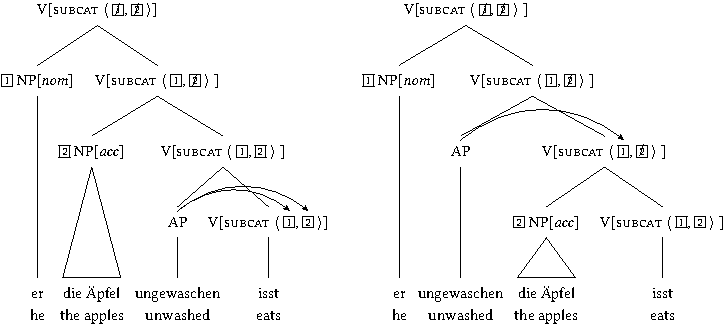
\includegraphics[width=\textwidth]{Figures/depictives-lsp-cropped.pdf}
%%  \resizebox{\linewidth}{!}{%
%% \begin{forest}
%% sn edges, for tree={l sep= 6ex}
%% [V{[\subcat \sliste{ \spirit{1}, \spirit{2} }]}
%% 	[\ibox{1} NP{[\textit{nom}]}
%% 		[er;he]]
%% 	[V{[\subcat \sliste{ \ibox{1}, \spirit{2} } ]}
%% 		[\ibox{2} NP{[\textit{acc}]}
%% 			[die Äpfel;the apples,triangle]]
%% 		[V{[\subcat \sliste{ \ibox{1}, \ibox{2} } ]}
%% 			[\subnode{ap1}{AP}
%% 				[ungewaschen;unwashed]]
%% 			[V{[\subcat \sliste{ \subnode{arg11}{\ibox{1}}, \subnode{arg12}{\ibox{2}} }]}
%% 				[isst;eats]]]]]
%% \end{forest}
%% \hspace{1em}
%% \begin{forest}
%% sn edges, for tree={l sep= 6ex}
%% [V{[\subcat \sliste{ \spirit{1}, \spirit{2} } ]}
%% 	[\ibox{1} NP{[\textit{nom}]}
%% 		[er;he]]
%% 	[V{[\subcat \sliste{ \ibox{1}, \spirit{2} } ]}
%% 		[\subnode{ap2}{AP}
%% 			[ungewaschen;unwashed]]
%% 		[V{[\subcat \sliste{ \subnode{arg21}{\ibox{1}}, \spirit{2} } ]}
%% 			[\ibox{2} NP{[\textit{acc}]}
%% 				[die Äpfel;the apples,triangle]]
%% 			[V{[\subcat \sliste{ \ibox{1}, \ibox{2} } ]}
%% 				[isst;eats]]]]]
%% \end{forest}
%% % This has to be inside of the scaling
%%     %% \begin{tikzpicture}[overlay,remember picture]
%%     %% %% this works with tikzmark
%%     %% \draw[->, bend angle=40, bend left] ($(pic cs:ap1)+(1ex,2ex)$) to($(pic cs:arg11)+(1ex,2.5ex)$);
%%     %% \draw[->, bend angle=40, bend left] ($(pic cs:ap1)+(1ex,2ex)$) to($(pic cs:arg12)+(1ex,2.5ex)$); % 1ex links, 2ex hoch
%%     %% %
%%     %% \draw[->, bend angle=40, bend left] ($(pic cs:ap2)+(1ex,2ex)$) to($(pic cs:arg21)+(1ex,2.5ex)$);
%%     %% \end{tikzpicture}
%% % somehow it stopped working
%% %% this used to work with subnode in texlive 2013 but is broken now
%% \begin{tikzpicture}[overlay,remember picture] 
%% \draw[->, bend angle=40, bend left] (ap1.north) to (arg11.north);
%% \draw[->, bend angle=40, bend left] (ap1.north) to (arg12.north); 
%% %
%% \draw[->, bend angle=40, bend left] (ap2.north) to (arg21.north);
%% \end{tikzpicture}
%}
%\hfill\mbox{}
\caption{Analysis of \emph{dass er die Äpfel ungewaschen isst} `that he the apples unwashed eats' and \emph{dass er ungewaschen die
    Äpfel isst} `that he unwashed the apples eat'}\label{anal-er-die-frau-nackt-sieht}
\end{figure}%
Arguments that have been realized are still represented on the upper nodes, however, they are crossed"=out and thereby marked as ``realized''.
In German, this preference for the antecedent noun can be captured by assuming a restriction that states that the antecedent noun must not yet have been
realized.

It is commonly assumed for English\il{English} that adjuncts are combined with a VP.
\eal
\ex John [[\sub{VP} ate the apples$_i$] unwashed$_i$].
\ex You can't [[\sub{VP} give them$_i$ injections] unconscious$_i$].\footnote{
\citew[\page 17]{Simpson2003a}.
}
\zl
In approaches where the arguments of the verb are accessible at the VP node, it is possible to establish a relation between
the depictive predicate and an argument although the antecedent noun is inside the VP.
English differs from German in that depictives can refer to both realized (\emph{them} in (\mex{0}b))
and unrealized (\emph{you} in (\mex{0}b)) arguments.

\citet[\page 560]{Higginbotham85a} and \citet{Winkler97a} have proposed corresponding non"=cancellation approaches in \gbt.
There are also parallel suggestions in Minimalist theories: checked features are not deleted, but instead marked as already
checked \citep[\page 14]{Stabler2010b}. However, these features are still viewed as inaccessible.\label{page-non-cancellation-end}

Depending on how detailed the projected information is, it can be possible to see adjuncts and argument in embedded structures as well as their
phonological, syntactic and semantic properties. In the CxG variant proposed by Kay and Fillmore, all information is available. In LFG,
information about grammatical function, case and similar properties is accessible. However, the part of speech is not contained in the f"=structure.
If the part of speech does not stand in a one"=to"=one relation to grammatical function, it cannot be restricted using selection via f"=structure.
Nor is phonological information represented completely in the f"=structure. If the analysis of idioms requires nonlocal access to phonological
information or part of speech, then this has to be explicitly encoded in the f"=structure (see \citew[\page 46--50]{Bresnan82a} for more on idioms). 

In the HPSG variant that I adopt, only information about arguments is projected. Since arguments are always represented by descriptions of type
\type{synsem}, no information about their phonological realization is present. However, there are daughters in the structure so that it is still
possible to formulate restrictions for idioms as in TAG or Construction Grammar (see \citew{RS2009a}
for an analysis of the `horse' example in (\ref{ex-ich-glaube-mich-tritt-ein-Pferd})).
This may seem somewhat like overkill: although we already have the tree structure, we are still projecting information about arguments
that have already been realized (unfortunately these also contain information about their arguments and so on). At this point, one could be inclined
to prefer TAG or LFG since these theories only make use of one extension of locality: TAG uses trees
of arbitrary or rather exactly the necessary size and LFG makes reference to a complete
f"=structure. However, things are not quite that simple: if one wants to create a relation to an
argument when adjoining a depictive predicate in TAG, then one requires a list of
possible antecedents. Syntactic factors (\eg reference to dative vs.\ accusative noun phrases, to argument vs.\ adjuncts,
coordination of verbs vs.\ nouns) play a role in determining the referent noun, this cannot be reduced to semantic relations.
Similarly, there are considerably different restrictions for different kinds of idioms and these cannot all be formulated in terms of restrictions
on f"=structure since f"=structure does not contain information about parts of speech.\is{depictive predicate|)}

One should bear in mind that some phenomena require reference to larger portions of structure. The majority of phenomena can be treated in terms of head
domains and extended head domains, however, there are idioms that go beyond the sentence level. Every theory has to account for this somehow.
\is{locality|)}\is{idiom|)}



%      <!-- Local IspellDict: en_US-w_accents -->

%% -*- coding:utf-8 -*-
\section{Recursion}
\label{sec-recursion}

Every\is{recursion|(} theory in this book can deal with self"=embedding in language as it was
discussed on page~\pageref{ex-that-max-thinks-that-recursion}. The example
(\ref{ex-that-max-thinks-that-recursion}) is repeated here as (\mex{1}):
\ea
\label{ex-that-max-thinks-that-recursion-two}
that Max thinks [that Julia knows [that Otto claims [that Karl
suspects [that Richard confirms [that Friederike is laughing]]]]]
\z
Most theories
capture this directly with recursive phrase structure rules or dominance schemata. TAG\indextag is
special with regard to recursion since recursion is factored out of the trees. The corresponding
effects are created by an adjunction operation that allows any amount of material to be inserted
into trees.  It is sometimes claimed that Construction Grammar\indexcxg cannot capture the existence
of recursive structure in natural language (\eg \citealp[\page 269]{Leiss2009a}).  This impression
is understandable since many analyses are extremely surface"=oriented. For example, one often talks
of a [Sbj TrVerb Obj] construction. However, the grammars in question also become recursive as soon
as they contain a sentence embedding or relative clause construction. A sentence embedding
construction could have the form [Sbj that-Verb that-S], where a that-Verb is one that can take
a sentential complement and that-S stands for the respective complement. A \emph{that}"=clause can then be inserted
into the that-S slot. Since this \emph{that}"=clause can also be the result of the application of
this construction, the grammar is able to produce recursive structures such as those in (\mex{1}):

\ea
Otto claims [\sub{that-S} that Karl suspects [\sub{that-S} that Richard sleeps]].
\z
In (\mex{0}), both \emph{Karl suspects that Richard sleeps} and the entire clause are instances of the [Sbj
that-Verb that-S] construction. The entire clause therefore contains an embedded subpart that is licensed by
the same construction as the clause itself. (\mex{0}) also contains a constituent of the category
\emph{that}-S that is embedded inside of \emph{that}-S. For more on recursion and self"=embedding\is{self"=embedding} in Construction Grammar, see \citew{Verhagen2010a}.

Similarly, every Construction Grammar that allows a noun to combine with a genitive\is{genitive} noun phrase also allows
for recursive structures. The construction in question could have the form [Det N
NP[gen] ] or [ N NP[gen] ]. The [Det N NP[gen] ] construction licenses structures such as (\mex{1}):
\ea
\gll [\sub{NP} des Kragens [\sub{NP} des Mantels [\sub{NP} der Vorsitzenden]]]\\
	{} the collar {} of.the coat {} of.the chairwoman\\
\glt `the collar of the coat of the chairwoman'
\z
\citet{Jurafsky96a} and \citet*{BLT2009a} use probabilistic context"=free grammars\is{context"=free grammar!probabilistic (PCFG)} (PCFG) for a Construction Grammar parser
with a focus on psycholinguistic plausibility and modeling of acquisition. Context"=free grammars
have no problems with self"=embedding\is{self"=embedding} structures like those in (\mex{0}) and thus this kind
of Construction Grammar itself does not encounter any problems with self"=embedding.

\citet[\page 192]{Goldberg95a} assumes that the resultative construction\is{construction!resultative} for English\il{English} has the following
form:
\ea
{}[SUBJ [V OBJ OBL]] 
\z
This corresponds to a complex structure as assumed for elementary trees in TAG. LTAG differs from Goldberg's approach in that every structure requires a lexical
anchor, that is, for example (\mex{0}), the verb would have to be fixed in LTAG. But in Goldberg's analysis, verbs can be inserted into independently
existing constructions (see Section~\ref{Abschnitt-Stoepselei}). In TAG publications, it is often emphasized that elementary trees do not contain any recursion.
The entire grammar is recursive however, since additional elements can be added to the tree using adjunction and -- as (\mex{-2}) and
(\mex{-1}) show -- insertion into substitution nodes can also create recursive structures.
\is{recursion|)}



%      <!-- Local IspellDict: en_US-w_accents -->


%% Here’s Chomsky’s description of this fact in his (1964:7):
%% …a mature native speaker can produce a new sentence of his language on the appropriate occasion, and other speakers can understand it immediately, though it is equally new to them. Most of our linguistic experience, both as speakers and hearers, is with new sentences; once we have mastered a language, the class of sentences with which we can operate fluently is so vast that for all practical purposes (and, obviously, for all theoretical purposes), we may regard it as infinite.

